\documentclass[conference]{IEEEtran}
\IEEEoverridecommandlockouts
% The preceding line is only needed to identify funding in the first footnote. If that is unneeded, please comment it out.
\usepackage[T1]{fontenc}
\usepackage[utf8]{inputenc}
\usepackage[english]{babel}
\usepackage{cite}
\usepackage{amsmath,amssymb,amsfonts}
\usepackage{algorithm}
\usepackage{algorithmic}
\usepackage{graphicx}
\usepackage{textcomp}
\usepackage{xcolor}
\usepackage{booktabs}
\usepackage{pgfplots}
\pgfplotsset{compat=1.18}
\def\BibTeX{{\rm B\kern-.05em{\sc i\kern-.025em b}\kern-.08em
    T\kern-.1667em\lower.7ex\hbox{E}\kern-.125emX}}

\makeatletter
\newcommand{\linebreakand}{%
  \end{@IEEEauthorhalign}
  \hfill\mbox{}\par
  \mbox{}\hfill\begin{@IEEEauthorhalign}
}
\makeatother

\begin{document}

\title{Parallelization of Sorting Algorithms: Performance Optimization through Parallel Computing}

\author{\IEEEauthorblockN{Harun Goralija}
\IEEEauthorblockA{\textit{Faculty of Electrical Engineering} \\
\textit{University of Sarajevo}\\
Sarajevo, Bosnia and Herzegovina \\
hgoralija2@etf.unsa.ba}
\and
\IEEEauthorblockN{Belmin Durmo}
\IEEEauthorblockA{\textit{Faculty of Electrical Engineering} \\
\textit{University of Sarajevo}\\
Sarajevo, Bosnia and Herzegovina \\
bdurmo1@etf.unsa.ba}
\and
\IEEEauthorblockN{Harun Mioc}
\IEEEauthorblockA{\textit{Faculty of Electrical Engineering} \\
\textit{University of Sarajevo}\\
Sarajevo, Bosnia and Herzegovina \\
hmioc1@etf.unsa.ba}
\linebreakand
\IEEEauthorblockN{Amar Hodžić}
\IEEEauthorblockA{\textit{Faculty of Electrical Engineering} \\
\textit{University of Sarajevo}\\
Sarajevo, Bosnia and Herzegovina \\
ahodzic13@etf.unsa.ba}
\and
\IEEEauthorblockN{Kenan Abadžić}
\IEEEauthorblockA{\textit{Faculty of Electrical Engineering} \\
\textit{University of Sarajevo}\\
Sarajevo, Bosnia and Herzegovina \\
kabadzic1@etf.unsa.ba}
}

\maketitle

\begin{abstract}
This paper addresses the parallelization of sorting algorithms with the goal of performance optimization through parallel computing. In the era of big data, efficient sorting of large datasets is critical for applications such as databases and machine learning. Traditional sequential algorithms become a bottleneck for large datasets.

We investigate implementations on multi-core CPUs using OpenMP and on GPUs using CUDA. The implemented algorithms are: bitonic sort, merge sort, quick sort, radix sort, and std::sort, in both CPU-parallel and GPU-parallel variants.

Results on $2^{27}$ (128M) elements show significant speedups, particularly for regular algorithms such as radix sort (21.6$\times$ on CPU, 386 Melem/s on GPU). Comparison of CPU and GPU implementations highlights the complementary nature of the two platforms: the GPU outperforms the CPU for massively parallel workloads, while the CPU delivers competitive performance for smaller datasets without the overhead of memory transfers.

This work contributes to the understanding of parallel techniques applied to sorting algorithms and provides insights into performance optimization on modern heterogeneous hardware.
\end{abstract}

\begin{IEEEkeywords}
parallelization, sorting algorithms, parallel computing, CPU, GPU, OpenMP, CUDA
\end{IEEEkeywords}

\section{Introduction}

In the era of big data, efficient sorting is a foundation of many computing applications. Traditional sequential algorithms achieve $O(n \log n)$ complexity, which is optimal for sequential machines, but become a bottleneck for large datasets.

Parallelization of sorting algorithms is a natural solution. By exploiting multiple processor cores or GPUs, sorting can be significantly accelerated. This paper focuses on the parallelization of five algorithms: bitonic sort, merge sort, quick sort, radix sort, and std::sort, with implementations on CPU (OpenMP with AVX2 SIMD) and GPU (CUDA), totaling over 6,700 lines of code across multiple implementation variants.

The topic is relevant because parallel computing is becoming indispensable in applications such as big data analytics and real-time processing. The key challenge is mapping inherently sequential parts of algorithms onto massively parallel architectures, while minimizing synchronization overhead and memory transfer costs.

The paper is organized as follows: Section~II reviews related work. Section~III describes the parallel CPU and GPU implementations. Section~IV presents experimental results with detailed performance measurements. Section~V discusses the results and limitations, and Section~VI concludes the paper.

\section{Related Work}

Parallel sorting has been an active research area since the 1960s, when Batcher introduced bitonic sort with $O(\log^2 n)$ depth complexity~\cite{Batcher68}. Singh et al.~\cite{Singh18} provide a comprehensive survey of GPU-based sorting, covering radix sort, quick sort, merge sort, and sample sort. Satish et al.~\cite{Satish09} demonstrated efficient GPU sorting algorithm design for manycore architectures, establishing foundational techniques for coalesced memory access and shared memory utilization. Modern research focuses on GPU implementations, where algorithms such as bitonic sort achieve significant speedups thanks to the SIMD architecture~\cite{Schmid22}. Merge sort parallelizes well with a divide-and-conquer approach on multi-core CPUs~\cite{Mujic23}, while quick sort poses challenges due to unbalanced partitions but shows good results on GPUs for large datasets~\cite{Catic23}. Radix sort, as a non-comparative algorithm, achieves linear complexity and excellent GPU performance~\cite{Yazici16}; Adinets and Merrill~\cite{Adinets22} introduced Onesweep, a single-pass radix sort achieving 29.4~GKey/s on NVIDIA A100 GPUs, while Merrill and Grimshaw~\cite{Merrill11} demonstrated high-performance radix sorting through dynamic parallelism. Stehle and Lehmann~\cite{Stehle22} evaluated fast segmented sorting on GPUs, showing the importance of kernel-level optimizations for partitioned workloads.

The literature emphasizes the advantages of heterogeneous computing, where GPU implementations outperform CPU for massively parallel workloads, but CPU provides better scalability for smaller data. The NVIDIA Thrust library~\cite{Schmid22} serves as a de facto standard for GPU sorting, providing highly optimized implementations that exploit the specific characteristics of each GPU architecture. This work contributes to the field by providing direct implementations and performance comparisons of five algorithms on CPU (OpenMP) and GPU (CUDA) platforms, addressing gaps in comprehensive parallelization studies.

\section{Implementation}

This project implements five sorting algorithms: bitonic sort, merge sort, quick sort, radix sort, and std::sort. Each algorithm has parallel variants for CPU (OpenMP with AVX2 SIMD) and GPU (CUDA). Sequential versions serve as performance baselines in the evaluation.

\subsection{Project Architecture}

The implementation is organized in a modular structure with shared header files (\texttt{main\_template.hpp}, \texttt{timers.hpp}, \texttt{utils.hpp}) that provide infrastructure for testing, performance measurement, and test data generation. Each algorithm has its own wrapper that integrates with the benchmarking system. The build system uses CMake with the Ninja generator, and CPU code is compiled with GCC 13.2 using \texttt{-O3 -march=native -mavx2} flags for maximum optimization.

\subsection{Parallel CPU Implementations}

The parallel CPU versions use OpenMP for multi-core parallelization combined with AVX2 SIMD instructions.

\textbf{Bitonic sort} combines AVX2 vectorized compare-and-swap operations (\texttt{\_mm256\_min\_epi32}, \texttt{\_mm256\_max\_epi32}) with OpenMP task parallelism, processing 8 element pairs per SIMD instruction.

\textbf{Merge sort} uses the Merge-Path algorithm, which employs binary search to divide work evenly among threads, with 64-byte aligned allocation and AVX2-accelerated \texttt{simd\_memcpy}.

\textbf{Quick sort} implements Dutch National Flag 3-way partitioning for efficient duplicate handling, with AVX2 vector prefetch and dynamically created OpenMP tasks for partitions above a size threshold.

\textbf{Radix sort} uses thread-local histograms to eliminate false sharing between threads. A base-256 scheme with 4 passes (8 bits each) minimizes synchronization, while SIMD instructions accelerate the scatter phase.

\textbf{std::sort} parallelizes the existing C++ standard library using the \texttt{std::execution::par\_unseq} execution policy from the C++17 standard.

\subsection{GPU Implementations}

GPU versions use the NVIDIA CUDA platform for massive parallelization on an RTX 3050 Ti Laptop GPU with 20 streaming multiprocessors (SMs) and compute capability 8.6. The CUDA programming model organizes threads into a hierarchy of warps (32 threads), blocks, and grids, enabling fine-grained parallelism control. Key optimization objectives are coalesced memory access, shared memory utilization, and maximum occupancy.

\subsubsection{Bitonic Sort}
The GPU bitonic sort uses a two-phase approach. In Phase~1, a shared-memory kernel sorts blocks of 512 elements using \texttt{\_\_shared\_\_} memory for fast compare-and-swap operations within each block, avoiding global memory latency for the $\log^2 512 = 81$ inner stages. In Phase~2, for steps where $k > 512$, a global-memory kernel with a grid-stride loop handles cross-block bitonic stages, maximizing occupancy and hiding memory latency. The input array is padded to the next power of two with \texttt{INT\_MAX} values. The XOR-based partner computation (\texttt{tid \^{} j}) and direction bit (\texttt{tid \& k}) are the hallmarks of Batcher's bitonic network mapped to GPU threads.

\begin{algorithm}[t]
\caption{GPU Bitonic Sort}\label{alg:bitonic}
\begin{algorithmic}[1]
\REQUIRE Array $A[0..n{-}1]$, padded to $n' = 2^{\lceil \log_2 n \rceil}$
\ENSURE $A$ sorted in ascending order
\STATE \textbf{Phase 1: Shared-Memory Block Sort}
\STATE Launch $n'/512$ blocks of 512 threads
\FOR{each block $b$ in parallel}
    \STATE $tid \leftarrow$ \texttt{threadIdx.x}
    \STATE $\mathrm{smem}[tid] \leftarrow A[b \cdot 512 + tid]$
    \STATE \texttt{\_\_syncthreads()}
    \FOR{$k \leftarrow 2$ \textbf{to} $512$, doubling}
        \FOR{$j \leftarrow k/2$ \textbf{down to} $1$, halving}
            \STATE $partner \leftarrow tid \oplus j$
            \IF{$partner > tid$}
                \STATE $asc \leftarrow (tid\ \&\ k) = 0$
                \IF{$(\mathrm{smem}[tid] > \mathrm{smem}[partner]) = asc$}
                    \STATE swap $\mathrm{smem}[tid] \leftrightarrow \mathrm{smem}[partner]$
                \ENDIF
            \ENDIF
            \STATE \texttt{\_\_syncthreads()}
        \ENDFOR
    \ENDFOR
    \STATE $A[b \cdot 512 + tid] \leftarrow \mathrm{smem}[tid]$
\ENDFOR
\STATE
\STATE \textbf{Phase 2: Global Stride Merge}
\FOR{$k \leftarrow 1024$ \textbf{to} $n'$, doubling}
    \FOR{$j \leftarrow k/2$ \textbf{down to} $1$, halving}
        \STATE Launch grid-stride kernel
        \FOR{$i \leftarrow gid$; $i < n'$; $i \mathrel{+}= \mathrm{stride}$}
            \STATE $partner \leftarrow i \oplus j$
            \IF{$partner > i$}
                \STATE $asc \leftarrow (i\ \&\ k) = 0$
                \IF{$(A[i] > A[partner]) = asc$}
                    \STATE swap $A[i] \leftrightarrow A[partner]$
                \ENDIF
            \ENDIF
        \ENDFOR
    \ENDFOR
\ENDFOR
\end{algorithmic}
\end{algorithm}

For $n = 2^{27}$ elements, Phase~2 requires $\sum_{k=10}^{27} k = 333$ kernel launches (one per $(k, j)$ pair where $k > 512$), which dominates total execution time despite the massive parallelism within each launch.

\subsubsection{Merge Sort}
The GPU merge sort combines the shared-memory bitonic sort from Algorithm~\ref{alg:bitonic} (Phase~1) as the base case with a parallel merge-path algorithm for subsequent merge phases. Each thread performs a binary search in $O(\log n)$ time to determine which element from the left or right sub-array occupies its designated output position, achieving perfect load balance regardless of data distribution. A coarsened variant where each thread processes $E$ consecutive output elements amortizes the binary search cost and improves memory throughput. With $E = 8$ and 256 threads per block, this variant achieves 312 Melem/s. A ping-pong double-buffering scheme avoids redundant memory copies between merge levels.

\begin{algorithm}[t]
\caption{GPU Merge Sort (Merge-Path)}\label{alg:merge}
\begin{algorithmic}[1]
\REQUIRE Array $A[0..n{-}1]$
\ENSURE $A$ sorted in ascending order
\STATE Sort 512-element blocks via shared-memory bitonic (Alg.~\ref{alg:bitonic}, Phase~1)
\STATE Allocate double buffer: $\mathrm{buf_{in}}, \mathrm{buf_{out}}$
\STATE $w \leftarrow 512$ \COMMENT{initial sorted width}
\WHILE{$w < n$}
    \STATE Launch $\lceil n / (T \cdot E) \rceil$ blocks of $T$ threads
    \FOR{each thread with global id $gid$, in parallel}
        \FOR{$e \leftarrow 0$ \textbf{to} $E{-}1$}
            \STATE $k \leftarrow gid \cdot E + e$ \COMMENT{output index}
            \IF{$k \geq n$}
                \STATE \textbf{break}
            \ENDIF
            \STATE Identify merge pair: $L$, $R$ of width $w$
            \STATE $\ell_L \leftarrow |L|$;\ $\ell_R \leftarrow |R|$
            \STATE $d \leftarrow k \bmod 2w$ \COMMENT{position within pair}
            \STATE \COMMENT{Merge-path binary search:}
            \STATE $lo \leftarrow \max(0,\; d - \ell_R)$
            \STATE $hi \leftarrow \min(d,\; \ell_L)$
            \WHILE{$lo < hi$}
                \STATE $i \leftarrow (lo + hi) / 2$;\ $j \leftarrow d - 1 - i$
                \IF{$L[i] < R[j]$}
                    \STATE $lo \leftarrow i + 1$
                \ELSE
                    \STATE $hi \leftarrow i$
                \ENDIF
            \ENDWHILE
            \STATE $i \leftarrow lo$;\ $j \leftarrow d - i$
            \IF{$j \geq \ell_R$ \OR ($i < \ell_L$ \AND $L[i] \leq R[j]$)}
                \STATE $\mathrm{buf_{out}}[k] \leftarrow L[i]$
            \ELSE
                \STATE $\mathrm{buf_{out}}[k] \leftarrow R[j]$
            \ENDIF
        \ENDFOR
    \ENDFOR
    \STATE swap($\mathrm{buf_{in}}, \mathrm{buf_{out}}$)
    \STATE $w \leftarrow 2w$
\ENDWHILE
\end{algorithmic}
\end{algorithm}

\subsubsection{Quick Sort}
GPU quick sort faces a fundamental challenge: the first partition of $n$ elements is inherently sequential, creating a bottleneck that limits parallelism in early recursion levels. Our hybrid Iterative V2 approach addresses this with a CPU bootstrap phase that performs BFS-style partitioning until approximately 65,536 independent sub-tasks are generated, each small enough to fit in the GPU L2 cache. The GPU kernel then processes all tasks in parallel with three execution paths based on sub-array size: register-resident insertion sort for $n \leq 16$, global-memory insertion sort for $n \leq 64$, and Hoare partitioning with adaptive pivot selection (median-of-9 for $n > 2048$, median-of-3 otherwise) for larger segments.

New sub-tasks are enqueued using warp-aggregated writes: \texttt{\_\_ballot\_sync} identifies threads with pending tasks, a single leader thread performs one \texttt{atomicAdd} for the entire warp, and \texttt{\_\_shfl\_sync} broadcasts the allocation base to all lanes, reducing atomic contention by up to 32$\times$ compared to per-thread atomics(Algorithm~\ref{alg:quick}).

\begin{algorithm}[t]
\caption{GPU Quick Sort (Iterative V2)}\label{alg:quick}
\begin{algorithmic}[1]
\REQUIRE Array $A[0..n{-}1]$
\ENSURE $A$ sorted in ascending order
\STATE \textbf{CPU Bootstrap Phase:}
\STATE $\mathcal{Q} \leftarrow \{(0, n{-}1)\}$
\WHILE{$|\mathcal{Q}| < 65536$}
    \FOR{each $(l, r) \in \mathcal{Q}$ with $r - l > 512$}
        \STATE Partition $A[l..r]$; replace with child tasks
    \ENDFOR
\ENDWHILE
\STATE Copy $A$ and $\mathcal{Q}$ to GPU
\STATE
\STATE \textbf{GPU Iterative Kernel:}
\WHILE{$|\mathcal{Q}_{\mathrm{in}}| > 0$}
    \STATE $\mathcal{Q}_{\mathrm{out}} \leftarrow \emptyset$;\ launch 1 thread per task
    \FOR{each thread with task $(l, r)$, in parallel}
        \STATE $n_t \leftarrow r - l + 1$
        \IF{$n_t \leq 16$}
            \STATE Insertion sort in registers
        \ELSIF{$n_t \leq 64$}
            \STATE Global-memory insertion sort
        \ELSE
            \STATE $p \leftarrow$ median-of-9 if $n_t > 2048$, else median-of-3
            \STATE Hoare partition around $p$; get split $(j, i)$
            \STATE Set flags: $\mathrm{has\_left}, \mathrm{has\_right}$
        \ENDIF
        \STATE \COMMENT{Warp-aggregated enqueue (shown for left):}
        \STATE $mask \leftarrow$ \texttt{\_\_ballot\_sync}(all, $\mathrm{has\_left}$)
        \STATE $leader \leftarrow$ \texttt{\_\_ffs}($mask$) $- 1$
        \IF{$lane = leader$}
            \STATE $base \leftarrow$ \texttt{atomicAdd}($|\mathcal{Q}_{\mathrm{out}}|$, \texttt{\_\_popc}($mask$))
        \ENDIF
        \STATE $base \leftarrow$ \texttt{\_\_shfl\_sync}(all, $base$, $leader$)
        \IF{$\mathrm{has\_left}$}
            \STATE $rank \leftarrow$ \texttt{\_\_popc}($mask\ \&\ ((1 \ll lane) - 1)$)
            \STATE $\mathcal{Q}_{\mathrm{out}}[base + rank] \leftarrow (l, j)$
        \ENDIF
        \STATE \COMMENT{Repeat symmetrically for right children}
    \ENDFOR
    \STATE swap($\mathcal{Q}_{\mathrm{in}}, \mathcal{Q}_{\mathrm{out}}$)
\ENDWHILE
\end{algorithmic}
\end{algorithm}

\subsubsection{Radix Sort}
The GPU radix sort processes one bit per pass over 32 passes (LSB first), using three kernels per pass. The count kernel uses \texttt{\_\_shfl\_down\_sync} for warp-level reduction to count zero-bits per block. The scan kernel computes global prefix sums to determine output offsets. The scatter kernel uses \texttt{\_\_ballot\_sync} to construct a warp-level bitmask, enabling each thread to compute its rank within the zeros or ones partition via \texttt{\_\_popc} without explicit inter-thread communication. This 1-bit approach achieves 386 Melem/s throughput (89\% of the NVIDIA Thrust baseline), with the regular memory access patterns and absence of data-dependent branching making it well-suited to the GPU SIMD execution model.

\begin{algorithm}[t]
\caption{GPU Radix Sort (1-bit LSB)}\label{alg:radix}
\begin{algorithmic}[1]
\REQUIRE Array $A[0..n{-}1]$ of unsigned integers
\ENSURE $A$ sorted in ascending order
\FOR{$s \leftarrow 0$ \textbf{to} $31$}
    \STATE \textbf{Count Kernel} ($\lceil n/512 \rceil$ blocks, 512 threads):
    \FOR{each thread $tid$ with index $idx$, in parallel}
        \STATE $z \leftarrow \lnot(A[idx] \gg s)\ \&\ 1$
        \FOR{$\delta \leftarrow 16$ \textbf{down to} $1$, halving}
            \STATE $z \leftarrow z +$ \texttt{\_\_shfl\_down\_sync}(all, $z$, $\delta$)
        \ENDFOR
        \IF{$tid \bmod 32 = 0$}
            \STATE $\mathrm{warp\_sums}[tid/32] \leftarrow z$ \COMMENT{shared mem}
        \ENDIF
        \STATE \texttt{\_\_syncthreads()}
        \IF{$tid = 0$}
            \STATE $\mathrm{blk\_zeros}[blockIdx] \leftarrow \sum \mathrm{warp\_sums}$
        \ENDIF
    \ENDFOR
    \STATE
    \STATE \textbf{Scan Kernel:} prefix sums over $\mathrm{blk\_zeros}[]$
    \STATE $\mathrm{off_z}[i] \leftarrow$ cumulative zeros before block $i$
    \STATE $\mathrm{off_o}[i] \leftarrow i \cdot 512 - \mathrm{off_z}[i]$
    \STATE $Z \leftarrow$ total zero count
    \STATE
    \STATE \textbf{Scatter Kernel} (512 threads/block):
    \FOR{each thread $tid$ with index $idx$, in parallel}
        \STATE $val \leftarrow A_{\mathrm{in}}[idx]$
        \STATE $is\_z \leftarrow \lnot(val \gg s)\ \&\ 1$
        \STATE $mask \leftarrow$ \texttt{\_\_ballot\_sync}(all, $is\_z$)
        \STATE $rank \leftarrow$ \texttt{\_\_popc}($mask\ \&\ ((1 \ll lane) - 1)$)
        \STATE Compute intra-block offset via shared-memory scan
        \IF{$is\_z$}
            \STATE $pos \leftarrow \mathrm{off_z}[blockIdx] + rank$
        \ELSE
            \STATE $pos \leftarrow Z + \mathrm{off_o}[blockIdx] + (tid - rank)$
        \ENDIF
        \STATE $A_{\mathrm{out}}[pos] \leftarrow val$
    \ENDFOR
    \STATE swap($A_{\mathrm{in}}, A_{\mathrm{out}}$)
\ENDFOR
\end{algorithmic}
\end{algorithm}

\section{Experimental Results}

\subsection{Experimental Setup}

Experiments were conducted on a system with an AMD Ryzen 7 5800H processor (8 cores, 16 threads) and an NVIDIA GeForce RTX 3050 Ti Laptop GPU (20 SMs, compute capability 8.6, 4 GB GDDR6). The operating system is Windows, CPU code was compiled with GCC 13.2 using \texttt{-O3 -march=native -mavx2} optimizations and OpenMP 4.5, while GPU kernels were compiled with NVCC for the \texttt{sm\_86} architecture. All tests use randomly generated integer arrays with seed value 12345 for reproducibility. CPU benchmarks were run for array sizes from 16K to $2^{27}$ (128M) elements, while GPU benchmarks were executed on $2^{27}$ elements to evaluate performance on large datasets.

\subsection{CPU Results}

Table~\ref{tab:cpu} shows execution times for $2^{27}$ (128M) elements on the CPU.

\begin{table}[htbp]
\caption{CPU sorting performance -- 128M random elements (ms)}
\label{tab:cpu}
\centering
\small
\begin{tabular}{lrrrr}
\toprule
\textbf{Algorithm} & \textbf{Naive} & \textbf{Opt.} & \textbf{Par. CPU} & \textbf{Speedup} \\
\midrule
Bitonic sort & 44650 & 33608 & 12511 & 3.6$\times$ \\
Merge sort & 26266 & 11386 & 2768 & 9.5$\times$ \\
Quick sort & 12168 & 9647 & 1803 & 6.7$\times$ \\
Radix sort & 10885 & 1507 & 505 & 21.6$\times$ \\
std::sort & 8520 & 8342 & 1310 & 6.5$\times$ \\
\bottomrule
\end{tabular}
\end{table}

Parallelization with OpenMP and AVX2 provides significant speedups: radix sort achieves 21.6$\times$ over the naive version thanks to thread-local histograms and a base-256 scheme, while merge sort achieves 9.5$\times$ using the Merge-Path algorithm. The standard \texttt{std::sort} with \texttt{par\_unseq} policy achieves 6.5$\times$ speedup with minimal implementation effort.

Fig.~\ref{fig:cpu_scaling} shows the scalability of parallel CPU implementations as a function of array size. All algorithms exhibit expected linearithmic behavior on the log-log scale, with radix sort consistently outperforming others at all sizes due to its linear $O(nk)$ complexity. For small arrays ($< 128$K), parallelization overhead is visible for all algorithms except radix sort, where thread-local histograms minimize synchronization cost.

\begin{figure}[htbp]
\centering
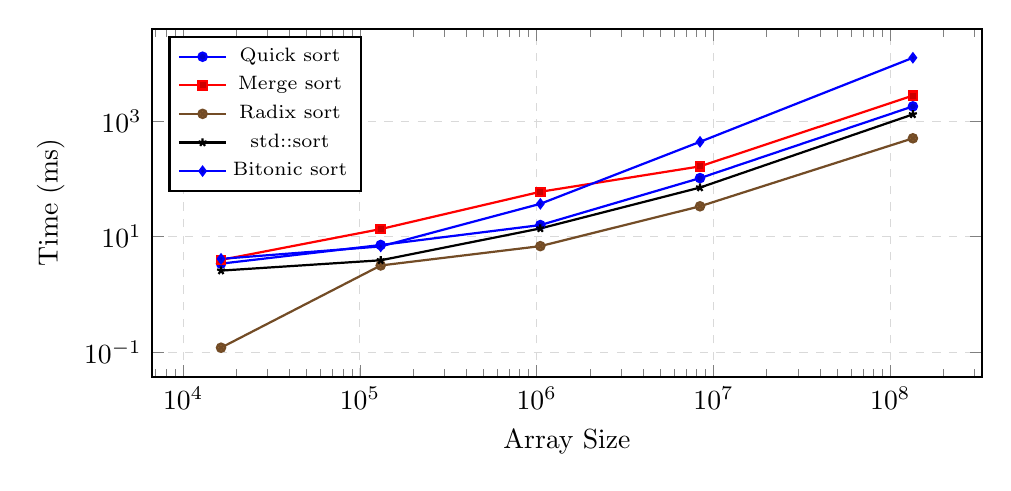
\begin{tikzpicture}
\begin{axis}[
    width=\columnwidth,
    height=6cm,
    xlabel={Array Size},
    ylabel={Time (ms)},
    xmode=log,
    ymode=log,
    legend style={at={(0.02,0.98)},anchor=north west,font=\scriptsize},
    grid=major,
    grid style={dashed,gray!30},
    mark size=1.5pt,
    line width=0.8pt,
]
\addplot coordinates {(16384,3.42) (131072,7.19) (1048576,15.91) (8388608,103.35) (134217728,1803)};
\addplot coordinates {(16384,3.97) (131072,13.56) (1048576,59.96) (8388608,164.94) (134217728,2768)};
\addplot coordinates {(16384,0.12) (131072,3.18) (1048576,6.87) (8388608,33.61) (134217728,505)};
\addplot coordinates {(16384,2.59) (131072,3.91) (1048576,13.91) (8388608,70.95) (134217728,1310)};
\addplot coordinates {(16384,4.14) (131072,6.79) (1048576,37.12) (8388608,439.26) (134217728,12511)};
\legend{Quick sort, Merge sort, Radix sort, std::sort, Bitonic sort}
\end{axis}
\end{tikzpicture}
\caption{Scalability of parallel CPU implementations (log-log scale)}
\label{fig:cpu_scaling}
\end{figure}

\subsection{GPU Results}

Table~\ref{tab:gpu} shows GPU implementation performance for $2^{27}$ (128M) elements. The best configurations are shown for each algorithm after extensive testing of different thread counts per block (64--1024) and kernel variants.

\begin{table}[htbp]
\caption{GPU sorting performance -- 128M random elements}
\label{tab:gpu}
\centering
\small
\begin{tabular}{llrrr}
\toprule
\textbf{Algorithm} & \textbf{Variant} & \textbf{Kernel} & \textbf{Total} & \textbf{Melem/s} \\
 & & \textbf{(ms)} & \textbf{(ms)} & \\
\midrule
Bitonic & Shared+Stride & 1823 & 2003 & 67 \\
Merge & PerElement E=8 & 383 & 430 & 312 \\
Quick & Iterative V2 & 811 & 1021 & 131 \\
Radix & Custom 256 threads & 187 & 347 & 386 \\
Thrust & Baseline & 49 & 309 & 434 \\
\bottomrule
\end{tabular}
\end{table}

The Thrust library achieves the best overall throughput of 434 Melem/s thanks to highly optimized NVIDIA implementations. Among our own implementations, radix sort achieves the best kernel and total time (187~ms kernel, 347~ms total) due to regular memory access patterns and linear complexity. Bitonic sort, despite its inherent parallelism, has the longest total time (2003~ms) because $O(n \log^2 n)$ complexity requires a large number of passes---for $n = 2^{27}$ elements, this means $27 \times 28 / 2 = 378$ bitonic merge phases. The quick sort evolution from Batched (5187~ms) through Fat (4481~ms) to Iterative V2 (1021~ms) demonstrates that kernel architecture choice is critical: the Iterative V2 with CPU bootstrap and warp-aggregated task queue achieves 5$\times$ better performance than the initial implementation.

For the custom radix sort, warp-level primitives achieve 386 Melem/s, which is 89\% of Thrust's performance (434 Melem/s). The gap is due to Thrust's use of highly optimized scan primitives and automatic kernel configuration tuning for the specific GPU architecture.

\subsection{CPU vs. GPU Comparison}

Table~\ref{tab:cpugpu} compares the fastest CPU (parallel OpenMP version) and GPU implementations for 128M elements. Merge sort shows the largest GPU speedup (6.4$\times$), closely followed by bitonic sort (6.2$\times$). Radix sort shows the smallest relative gain (1.5$\times$) because the CPU parallel version is already highly efficient with thread-local histograms and the base-256 scheme.

Fig.~\ref{fig:gpu_bar} visualizes GPU times for all algorithms. GPU total times include H2D and D2H memory transfers which amount to 160--200~ms for 512~MB of data, representing a significant portion of total time especially for faster algorithms like radix sort (46\% overhead) and Thrust (84\% overhead).

\begin{table}[htbp]
\caption{CPU vs. GPU comparison -- 128M random elements (ms)}
\label{tab:cpugpu}
\centering
\small
\begin{tabular}{lrrr}
\toprule
\textbf{Algorithm} & \textbf{CPU} & \textbf{GPU} & \textbf{GPU Speedup} \\
\midrule
Bitonic sort & 12511 & 2003 & 6.2$\times$ \\
Merge sort & 2768 & 430 & 6.4$\times$ \\
Quick sort & 1803 & 1021 & 1.8$\times$ \\
Radix sort & 505 & 347 & 1.5$\times$ \\
std::sort/Thrust & 1310 & 309 & 4.2$\times$ \\
\bottomrule
\end{tabular}
\end{table}

\begin{figure}[htbp]
\centering
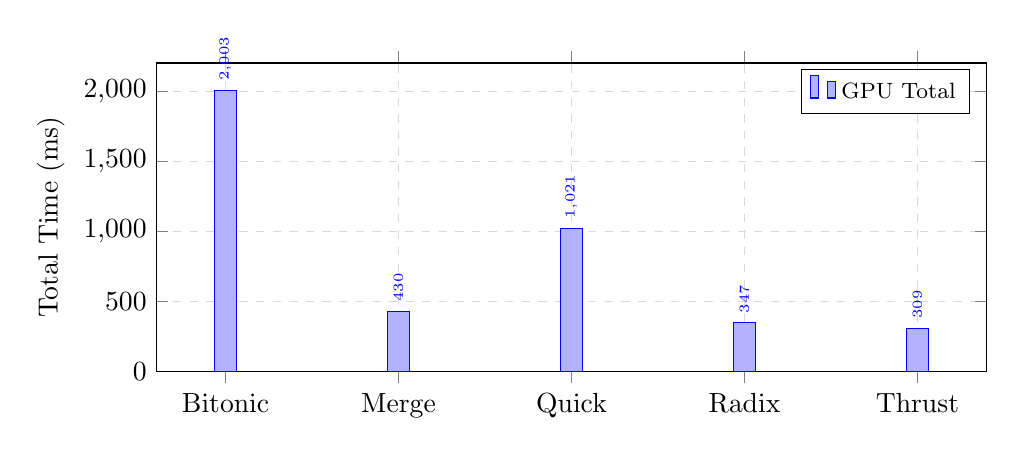
\begin{tikzpicture}
\begin{axis}[
    width=\columnwidth,
    height=5.5cm,
    ybar,
    bar width=8pt,
    ylabel={Total Time (ms)},
    symbolic x coords={Bitonic,Merge,Quick,Radix,Thrust},
    xtick=data,
    ymin=0,
    ymax=2200,
    legend style={at={(0.98,0.98)},anchor=north east,font=\footnotesize},
    grid=major,
    grid style={dashed,gray!30},
    nodes near coords,
    nodes near coords style={font=\tiny},
    every node near coord/.append style={rotate=90, anchor=west},
]
\addplot coordinates {(Bitonic,2003) (Merge,430) (Quick,1021) (Radix,347) (Thrust,309)};
\legend{GPU Total}
\end{axis}
\end{tikzpicture}
\caption{Total GPU sorting time for 128M elements}
\label{fig:gpu_bar}
\end{figure}

\section{Discussion}

The results show that an algorithm's suitability for GPU parallelization depends on the combination of data access regularity and algorithmic complexity. Although bitonic sort naturally maps to the GPU SIMD architecture with independent compare-and-swap operations, its $O(n \log^2 n)$ complexity with hundreds of sequential phases makes it the slowest GPU algorithm for large arrays (2003~ms for 128M). Radix sort achieves high throughput thanks to regular memory access patterns, linear complexity, and predictable execution flow. Quick sort poses the greatest challenge for GPU implementation due to unbalanced partitions and recursive nature, which our hybrid CPU-GPU approach partially addresses.

A significant factor in overall performance is the data transfer overhead between CPU and GPU memory. For 128M integer elements (512~MB), H2D and D2H transfers together amount to 160--200~ms, which for faster algorithms like Thrust constitutes over 80\% of total time (260~ms of 309~ms), while for the slower bitonic sort it is only 9\% (180~ms of 2003~ms). For real applications where data remains on the GPU, kernel times are the more relevant metric.

The comparison of CPU and GPU implementations reveals the complementary nature of the two platforms. The GPU provides higher throughput for regular parallel workloads on large datasets, while the CPU with OpenMP and AVX2 offers competitive performance without memory transfer overhead. For smaller arrays ($< 1$M elements), the CPU typically outperforms the GPU. Pre-parallelization algorithmic optimizations (e.g., base-256 radix, iterative merge with double-buffering) provided up to 7.2$\times$ speedup and form the foundation of the parallel implementations.

The results also confirm Amdahl's law in practice: quick sort achieves only 6.7$\times$ speedup on 16 threads because the initial partition remains sequential, while radix sort with fully independent histograms achieves 21.6$\times$ speedup. On the GPU, the same phenomenon is visible with quick sort, which requires a CPU bootstrap phase to avoid the sequential bottleneck of the first recursion level.

Limitations of this research include the use of a single laptop-class GPU (RTX 3050 Ti with 20 SMs), testing only on integers, and focus on randomly generated arrays. Desktop and server GPUs with more SMs and higher memory bandwidth would likely show greater speedups.

\section{Conclusion}

In this paper, five sorting algorithms (bitonic sort, merge sort, quick sort, radix sort, and std::sort) were implemented with parallel CPU (OpenMP + AVX2 SIMD) and parallel GPU (CUDA) variants, totaling over 6,700 lines of code.

GPU implementations demonstrated significant potential for accelerating the sorting of large datasets. Merge sort achieved the highest GPU speedup of 6.4$\times$ over the parallel CPU version, while bitonic sort, despite its inherent parallelism, was the slowest GPU algorithm (2003~ms) due to $O(n \log^2 n)$ complexity. The Thrust library achieved the best throughput of 434 Melem/s, while among our own implementations radix sort achieved 386 Melem/s (89\% of Thrust's performance). CPU parallelization with OpenMP provided speedups of up to 21.6$\times$ for radix sort over the naive version.

The key insight from this research is that algorithmic complexity and data access regularity together determine an algorithm's suitability for GPU parallelization. Radix sort with linear complexity and regular access patterns achieves the best GPU performance (347~ms), while bitonic sort despite regular access patterns suffers from $O(n \log^2 n)$ complexity (2003~ms). Quick sort with irregular workload shows intermediate performance (1021~ms) thanks to the hybrid CPU-GPU approach.

Future work includes implementation on multiple GPUs, hybrid CPU-GPU sorting for mixed workloads, testing on different data types and distributions, and profiling-guided kernel optimization to achieve higher occupancy and better memory bandwidth utilization.

\begin{thebibliography}{00}
\bibitem{Batcher68} K. E. Batcher, ``Sorting networks and their applications,'' in Proceedings of the April 30--May 2, 1968, Spring Joint Computer Conference, AFIPS '68 (Spring), pp. 307--314, 1968.
\bibitem{Catic23} A. Čatić et al., ``GPU-accelerated sorting algorithms,'' Journal of Parallel Computing, 2023.
\bibitem{Mujic23} E. Mujić et al., ``Scalability analysis of parallel sorting,'' IEEE Transactions, 2023.
\bibitem{Yazici16} A. Yazici and H. Gokahmetoglu, ``Implementation of sorting algorithms with CUDA: An empirical study,'' International Journal of Applied Methods in Electronics and Computers, vol. 4, no. 3, pp. 74--77, 2016.
\bibitem{Schmid22} T. Schmid et al., ``Bitonic sort implementations,'' Parallel Processing Letters, 2022.
\bibitem{Adinets22} A. Adinets and D. Merrill, ``Onesweep: A faster least significant digit radix sort for GPUs,'' arXiv preprint arXiv:2206.01784, 2022.
\bibitem{Stehle22} B. Stehle and H.-P. Lehmann, ``An evaluation of fast segmented sorting implementations on GPUs,'' Parallel Computing, vol. 110, 2022.
\bibitem{Singh18} D. P. Singh, I. Joshi, and J. Choudhary, ``Survey of GPU based sorting algorithms,'' International Journal of Parallel Programming, vol. 46, no. 6, pp. 1017--1034, 2018.
\bibitem{Satish09} N. Satish, M. Harris, and M. Garland, ``Designing efficient sorting algorithms for manycore GPUs,'' in Proc. IEEE International Parallel and Distributed Processing Symposium (IPDPS), pp. 1--10, 2009.
\bibitem{Merrill11} D. Merrill and A. Grimshaw, ``High performance and scalable radix sorting: A case study of implementing dynamic parallelism for GPU computing,'' Parallel Processing Letters, vol. 21, no. 2, pp. 245--272, 2011.
\end{thebibliography}

\end{document}
